\section{Deployment}
\subsection{Deployment Overview}
\begin{figure}[h!]
    \centering
    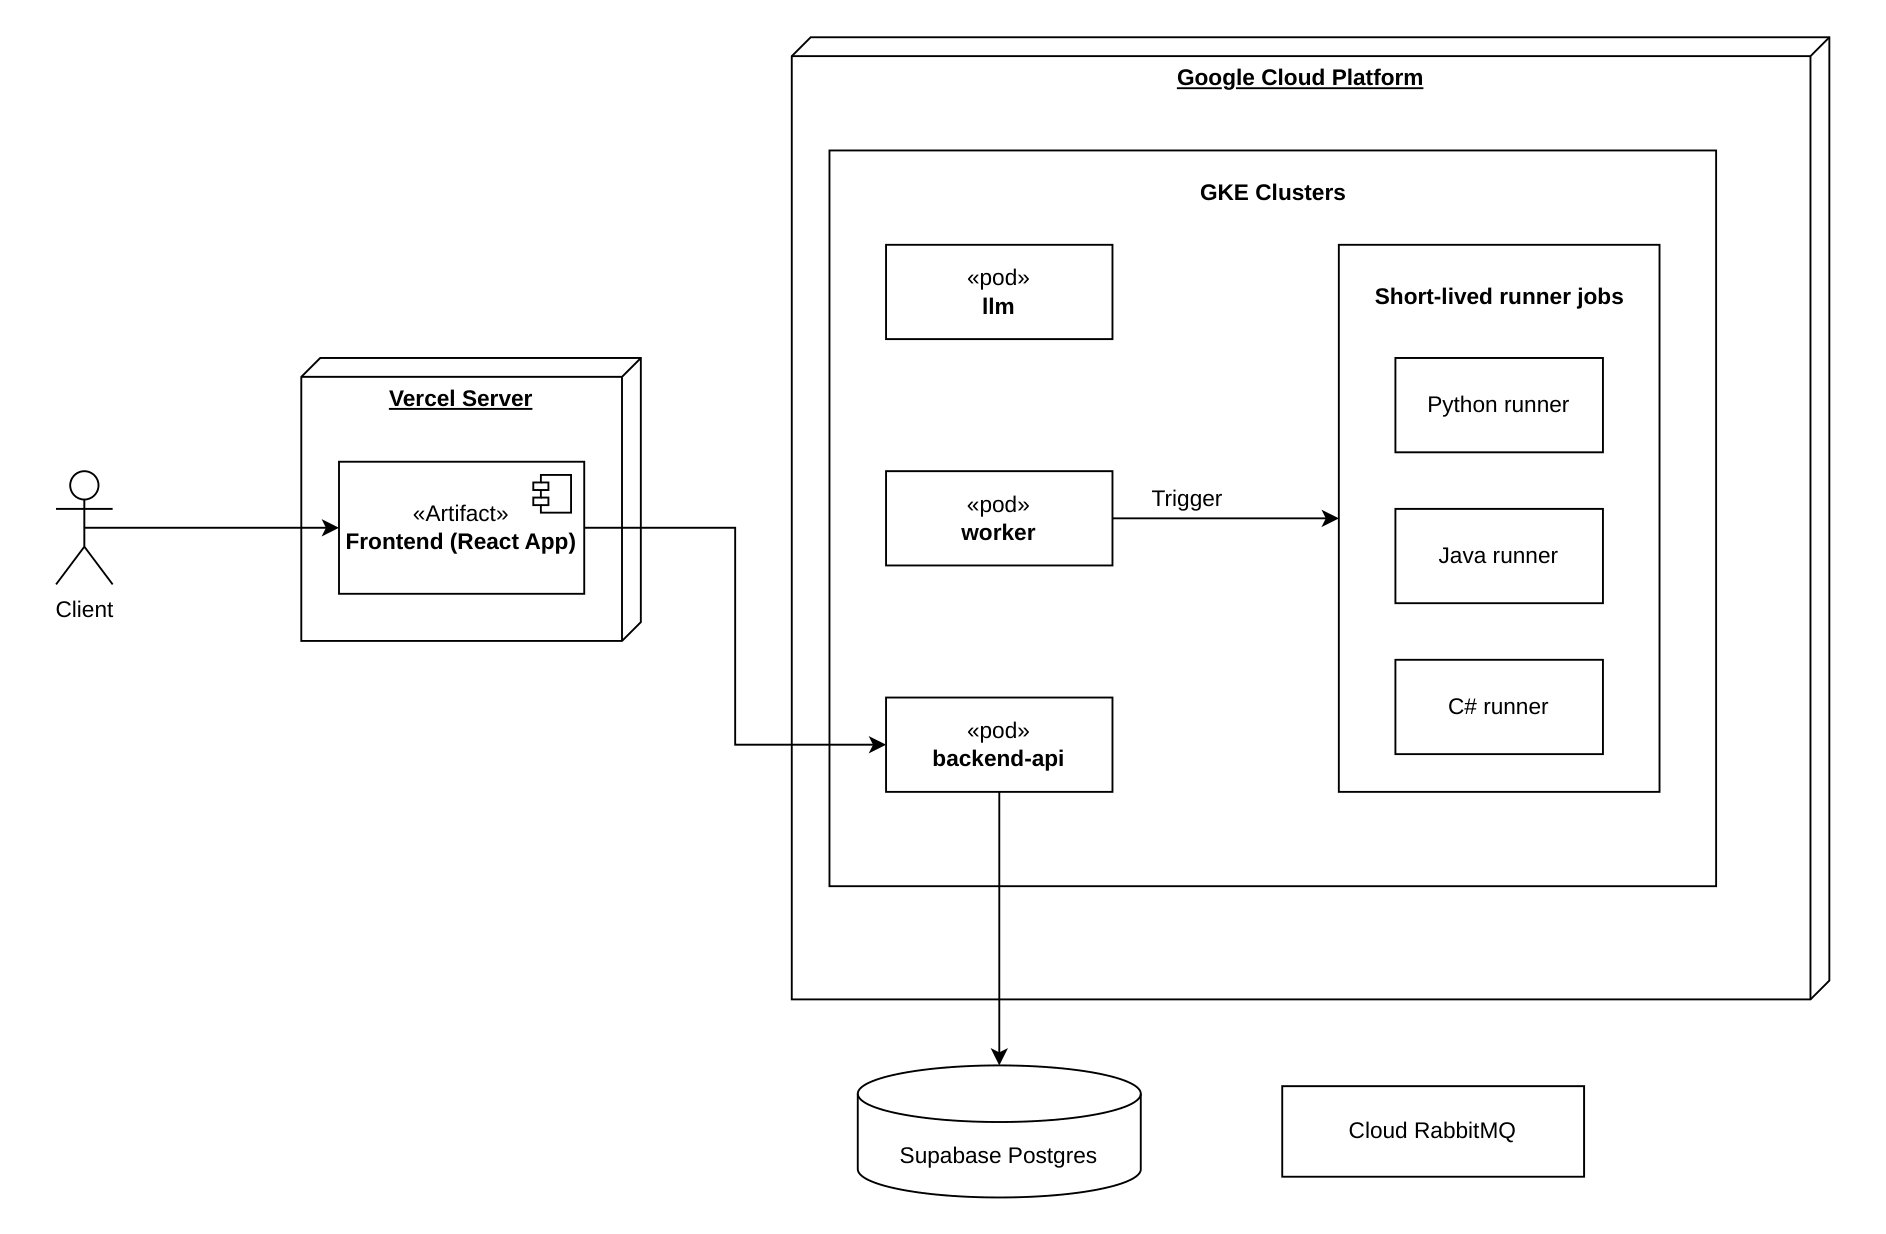
\includegraphics[width=1\textwidth]{Contents/Chapter 5/Deployment/deployment.png}
    \vspace{0.6cm}
    \caption{Deployment Diagram}
    \label{fig:deployment-diagram}
\end{figure}

The CodeRank system is deployed using a cloud-native architecture. Frontend application is deployed on Vercel because it provides simple hosting, automatic HTTPS, and continuous deployment for React/Vite applications. On the other hand, backend and worker services are deployed on Google Cloud using Google Kubernetes Engine (GKE), a managed Kubernetes platform for running containerized workloads. This separation allows the frontend to be optimized for static content delivery while the backend and code execution components are managed in an infrastructure environment designed for container orchestration.

While frontend is deployed through Vercel CI pipeline, the backend API, worker service, and programming language runners are containerized using Docker. Their images are stored in Google Artifact Registry, which is used as the private container registry for the project. The backend API runs as a long-running Kubernetes Deployment, while the worker service runs as an internal background Deployment that consumes messages from RabbitMQ. The language-specific code runners are not deployed as permanent services; instead, they are executed as short-lived Kubernetes Jobs created dynamically by the worker for each submission.

For data layer, the system uses Supabase, a managed backend service built on top of PostgreSQL. Supabase is the Postgres development platform \cite{supabase2026}. Supabase provides a fully managed relational database along with a suite of backend capabilities, making it a comprehensive platform for modern application development. For asynchronous communication between the services, the system uses RabbitMQ hosted on CloudAMQP. CloudAMQP provides managed RabbitMQ servers and clusters in the cloud, including monitoring tools, alarms, and management interfaces \cite{cloudamqp2026}. For AI related workflow, we utilize n8n cloud, a workflow automation platform that allows us to create and manage complex workflows integrating various services, including Google Gemini for the chatbot feature \cite{n8n2026}.


\subsection{Frontend Deployment}

The frontend of the CodeRank system is deployed on Vercel, a cloud platform designed for hosting modern web applications with a focus on performance, scalability, and developer experience. Vercel provides features such as automatic builds, global content delivery through an edge network, automatic HTTPS, and seamless integration with Git-based workflows. These capabilities make it well-suited for the React/Vite frontend used by CodeRank.

By leveraging Vercel, the frontend application benefits from automatic HTTPS, fast global content delivery, and continuous deployment. Every change pushed to the frontend repository can trigger an automated build and deployment process, ensuring that the latest version of the application is available without manual server management. The frontend communicates with the backend through HTTPS REST API requests. The backend base URL is configured as an environment variable, for example \texttt{VITE\_API\_URL}, so the same frontend codebase can be deployed to different environments.

The deployment process is straightforward and consists of the following steps:

\begin{itemize}
  \item Authentication: Log in to Vercel using a Git provider account such as GitHub.
  \item Repository Selection: Choose the repository containing the frontend application.
  \item Configuration and Deployment: Configure required environment variables such as the backend API endpoint and start the deployment process. Vercel then builds and deploys the application automatically.
\end{itemize}

Once deployed, the frontend is served via Vercel and communicates with the backend service exposed from Google Cloud. The production deployment of the CodeRank frontend is accessible at \url{https://code-rank-web.vercel.app/}.

\subsection{Backend and Worker Services Deployment}

\subsubsection{Google Cloud Platform Overview}

Google Cloud Platform (GCP) is a cloud computing platform that provides infrastructure and managed services for compute, networking, storage, databases, container orchestration, and application deployment \cite{google_cloud2026}. In this project, Google Cloud is selected for the backend and worker deployment because it provides a managed Kubernetes environment through Google Kubernetes Engine and a private image registry through Artifact Registry. These services match the system requirement of running both stable backend services and dynamic, per-submission code execution workloads.

Google Kubernetes Engine is used as the main runtime environment. GKE reduces the operational burden of managing Kubernetes clusters by providing managed control plane operations, node provisioning, workload scheduling, and integration with Google Cloud services. In particular, GKE Autopilot can manage node infrastructure, scaling, and resource configuration automatically, which is useful for a project where workload demand changes based on submission volume \cite{gke2026}. The backend API and worker are deployed as Kubernetes Deployments, while code execution is handled by Kubernetes Jobs. This model allows the system to run persistent services and temporary isolated execution tasks in the same platform.

Google Artifact Registry is used to store and manage Docker images for the backend, worker, and runner containers. Artifact Registry provides repositories for Docker and OCI images and integrates with Google Cloud runtimes such as GKE \cite{artifact_registry2026}. For CodeRank, this registry contains the following images:

\begin{itemize}
    \item \texttt{code-rank-backend}: the NestJS backend API image.
    \item \texttt{code-rank-worker}: the Go worker service image.
    \item \texttt{code-runner-python}: the Python code runner image.
    \item \texttt{code-runner-java}: the Java code runner image.
    \item \texttt{code-runner-csharp}: the C\# code runner image.
\end{itemize}

\subsubsection{Backend API Deployment}

The backend Deployment runs one or more replicas of the API container. Each replica listens on the configured application port and is exposed through a Kubernetes Service. In the initial deployment, a Service of type \texttt{LoadBalancer} can be used to provide a public endpoint for the Vercel frontend. In a production environment, this can be replaced or extended with an Ingress controller and a custom domain to provide HTTPS termination and cleaner routing.

The backend requires the following environment variables during deployment:

\begin{itemize}
    \item \texttt{DATABASE\_URL}: connection string of the managed PostgreSQL database.
    \item \texttt{RABBITMQ\_URI}: AMQP connection string provided by CloudAMQP.
    \item \texttt{CLIENT\_URL}: deployed Vercel frontend URL used for CORS configuration.
    \item \texttt{JWT\_ACCESS\_SECRET\_KEY} and \texttt{JWT\_REFRESH\_SECRET\_KEY}: secrets used for token generation.
    \item Third-party service credentials such as OAuth and Cloudinary credentials when enabled.
\end{itemize}

These values are stored in Kubernetes Secrets instead of being hard-coded in the container image. This design keeps application configuration separate from source code and allows the same backend image to be reused across development, staging, and production environments.

\subsubsection{Worker Service Deployment}

The worker service is a key component in the CodeRank deployment because it connects asynchronous submission processing with the Kubernetes-based code execution environment. Unlike the backend API, the worker does not expose a public HTTP endpoint. It runs as a background Deployment inside the GKE cluster and communicates with the rest of the system through RabbitMQ and the Kubernetes API.

The worker is implemented in Go and packaged as a Docker image. The image contains the compiled worker binary and the necessary runtime tools for interacting with Kubernetes. After being pushed to Artifact Registry, the worker image is deployed to GKE as a Kubernetes Deployment. The number of worker replicas can be adjusted based on submission traffic. Increasing the replica count allows multiple submissions to be consumed and processed in parallel, while RabbitMQ ensures that each message is delivered to one available consumer.

At runtime, the worker connects to CloudAMQP using the configured \texttt{RABBITMQ\_URI}. It consumes messages from the submission evaluation queue. Each message contains the submission code and execution metadata. After receiving a message, the worker performs the following steps:

\begin{enumerate}
    \item Parse the submission message from RabbitMQ.
    \item Fetch the testcase CSV file from the \texttt{testcaseUrl} included in the payload.
    \item Create a temporary runner configuration file containing the testcase path, timeout, memory limit, entry function, and submission identifier.
    \item Select the proper runner image based on the programming language, such as Python, Java, or C\#.
    \item Generate a Kubernetes ConfigMap containing the runner configuration, testcase CSV, and submitted source code.
    \item Create a Kubernetes Job that runs the selected language-specific runner image.
    \item Wait for the Job to finish and read the runner output from the Job logs.
    \item Convert the runner output into a submission result message and publish it back to RabbitMQ.
\end{enumerate}

The worker requires the following environment variables:

\begin{itemize}
    \item \texttt{RABBITMQ\_URI}: CloudAMQP connection string.
    \item \texttt{RUNNER\_EXECUTOR}: execution mode, set to \texttt{gke} in cloud deployment.
    \item \texttt{RUNNER\_K8S\_NAMESPACE}: namespace where runner Jobs are created.
    \item \texttt{RUNNER\_IMAGE\_PYTHON}: Artifact Registry image path for the Python runner.
    \item \texttt{RUNNER\_IMAGE\_JAVA}: Artifact Registry image path for the Java runner.
    \item \texttt{RUNNER\_IMAGE\_CSHARP}: Artifact Registry image path for the C\# runner.
\end{itemize}

Since the worker creates Kubernetes Jobs dynamically, it must be granted appropriate Kubernetes permissions. A dedicated Kubernetes ServiceAccount is assigned to the worker. This account is bound to a Role that allows creating ConfigMaps, creating Jobs, watching Jobs, and reading Pod logs in the runner namespace. This limits the worker permissions to only the resources needed for code execution.

\subsubsection{Runner Job Deployment Model}

The language-specific code runners are deployed differently from the backend and worker. They are not long-running services and do not require a Service or Ingress. Instead, each runner is stored as a Docker image in Artifact Registry. When a submission arrives, the worker creates a new Kubernetes Job using the correct runner image.

This execution model provides several advantages. First, each submission runs in a fresh container, reducing the risk of leftover state between submissions. Second, Kubernetes can enforce CPU, memory, and execution-time constraints at the Pod level. Third, the system can scale naturally because Kubernetes schedules runner Jobs based on available cluster capacity. Finally, completed Jobs can be removed automatically after a configured time-to-live value.

The runner Job receives three categories of input through a ConfigMap:

\begin{itemize}
    \item The submitted source code, mounted as the expected solution file for the selected language.
    \item The testcase CSV file fetched by the worker from remote storage.
    \item The runner configuration file, including timeout, memory limit, entry function, and submission identifier.
\end{itemize}

After execution, the runner writes a structured JSON result to its standard output. The worker reads the Job logs, extracts the JSON result, maps it to the backend submission result format, and publishes it to RabbitMQ. The backend then consumes the result message and updates the submission status in PostgreSQL.